\documentclass[11pt]{article}
\usepackage{bookmark}
\usepackage{algorithm}
\usepackage{algpseudocode}
\usepackage{amsfonts}
\usepackage{amsmath}
\usepackage{amssymb}
\usepackage{amsthm}
\usepackage{bm}
\usepackage{color}
\usepackage{comment}
\usepackage{float}
\usepackage{graphicx}
%\usepackage[hidelinks]{hyperref}
\usepackage{makecell}
\usepackage[caption=false,font=footnotesize,subrefformat=parens,labelformat=parens]{subfig}
\usepackage{wrapfig}
\usepackage{url}
\usepackage[table]{xcolor}
\graphicspath{{images_dd-mm2022/}}
\setlength{\parindent}{0.25in}
\setlength{\parskip}{.05in}
\pagestyle{plain}
%Title, date an author of the document
\title{Progress Report}
\author{Bardia Mojra}


\begin{document}
\maketitle
\thispagestyle{empty}

\bigskip
\bigskip
\begin{center}
 Robotic Vision Lab
\end{center}

\begin{center}
The University of Texas at Arlington
\end{center}

\newpage

\section{Specific Research Goals}
\begin{itemize}
      \item VPQEKF (\textcolor{red}{May 30th}): Work on the paper.
      \item DLO Manipulation Dataset (ICRA - \textcolor{red}{Sept. 1st})
\end{itemize}

\section{To Do}
\begin{itemize}
  \item QEKF Paper - 30\% extension (\textcolor{red}{June 30th}):
  \begin{itemize}
      \item Read and summarize recent VO and QEKF papers.
  \end{itemize}
  \item QEKF/QuEst+VEst Implementation (\textcolor{red}{May 30th}):
  \begin{itemize}
      \item Point-feature extraction: tracking issue
      \item Address scale factor (depth-scale) issues: DL solutions?
      \item Noise issue: noise cannot be modeled - revisit
      \item Adding plots - On-going
      \item Add semantic segmentation for detecting moving object pixels and rejecting matched features in those regions
  \end{itemize}
  \item  DLO Manipulation:  \textcolor{red}{ICRA - Sept. 1st}
  \begin{itemize}
      \item Find other ICRA dataset papers and summarize the structure. --- On-going.
      \item Dynamic Dataset Collection System with Reinforcement Learning:
      \begin{itemize}
        \item Design dynamic DLO data collection system.
        \item Build work cell.
        \item Collect data and create a dataset.
        \item Define evaluation metrics.
        \item Create a high frequency RGBD dataset with UV-frames and open-loop input control actions as the ground truth.
      \end{itemize}
      \item Real-Time Preception
      \begin{itemize}
        \item Deep learning methods for keypoint pose estimation in real-time.
        \item Use UV dye dataset
        \item Use PVNet-based approach for known-objects
      \end{itemize}
      \item Learning DLO Dynamics and System Identification
      \begin{itemize}
            \item List feasible approached for learing DLO dynamics
            \item Model dynamics and deformity in a latent space
      \end{itemize}
      \item Real-Time Control
      \begin{itemize}
        \item Time model inference, using auto-encoders generate the lowest
        dimensional representation for each object.
        \item Use another GAN model for object deformity for each object.
        \item Evaluate encoded representation for accuracy.
        \item Used another GAN to explore other abstraced representations from
        individual encoded representation. In theory, we can create a low
        dimensionsal representation for multiple similar objects, given all
        individual low-dimensional representations. This is inspired by "fundamental
        principles first" approach which has universal applicability.
      \end{itemize}
  \end{itemize}
\end{itemize}


\section{Progress}
The following items are listed in the order of priority:
\begin{itemize}
    \item XEst (\textcolor{red}{RAL - April 30st, 2022}): I found a series of
    papers on visual inertial odometry (VIO) and line feature tracking. In the VIO
    papers, the authors used inertial information from an IMU sensor to estimate
    depth. Per my conversation with Dr. Gans, we are not  interested in methods
    that use inertial information collected from an IMU as it would dilute our
    work on vision-based approaches. Moreover, line-feature tracking has been
    used in visual-SLAM applications and is shown to perform more robustly than
    line features. I have not found a working implementation yet. At this moment,
    I am redoing a part data log visualization for QEKF module.

    \begin{figure}[H]
      \begin{center}
        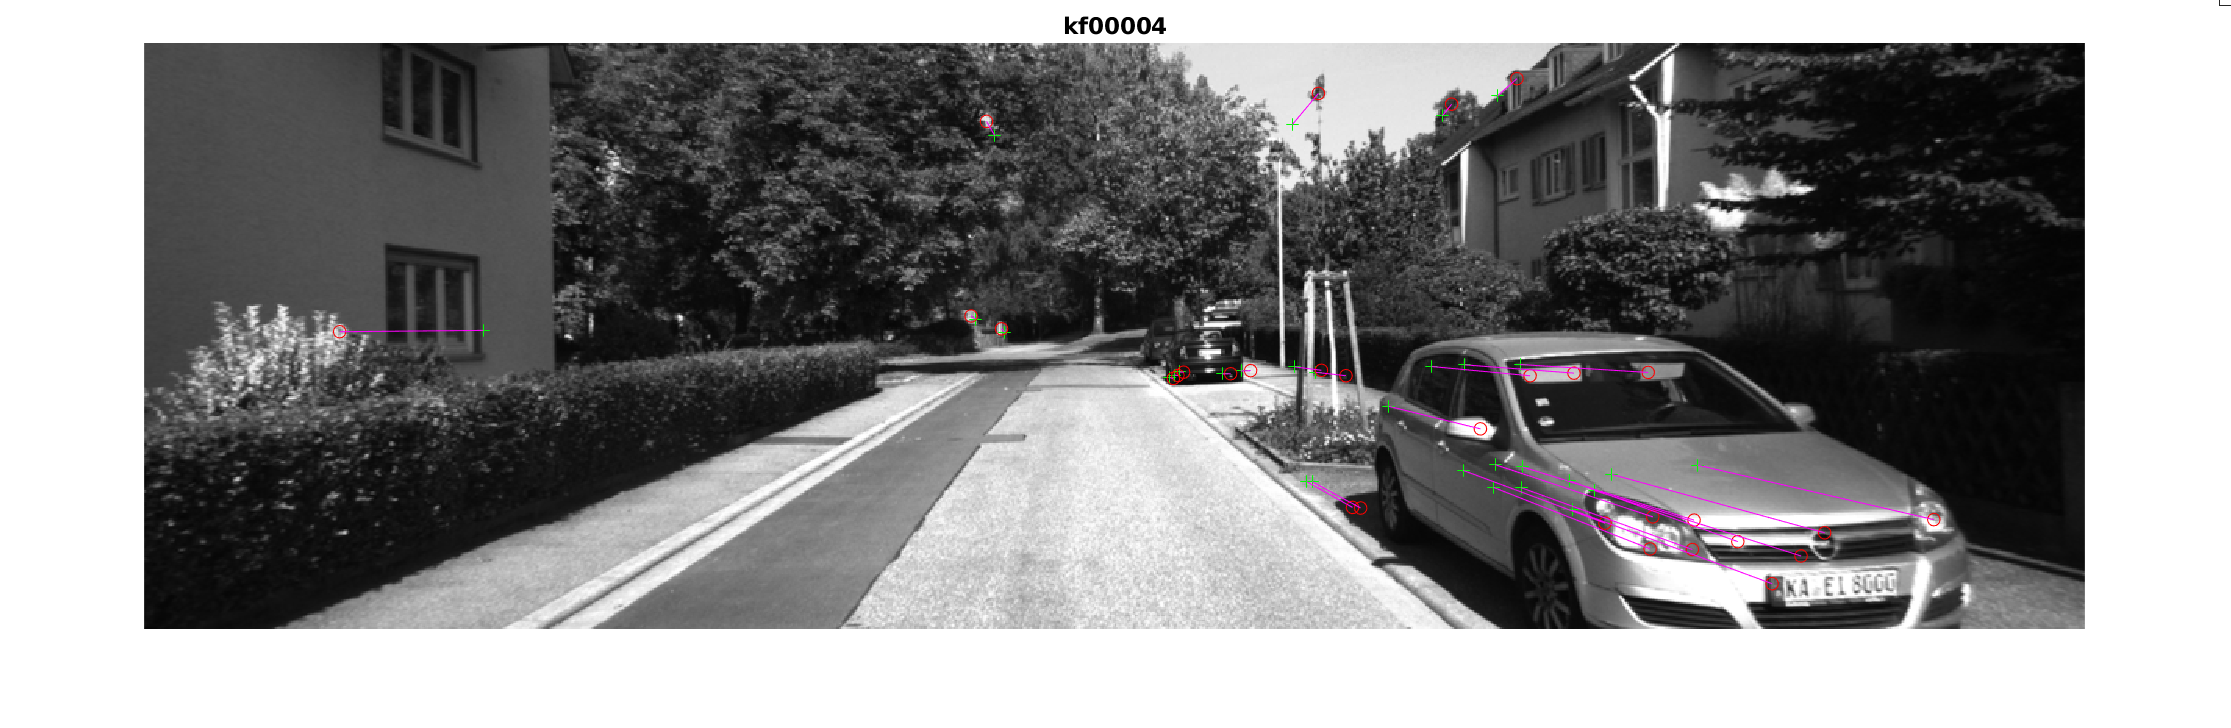
\includegraphics[width=\linewidth]{fig_mat-feat_kf00004.png}
      \end{center}
      \caption{Acceptable point-feature matches between two frames.}
    \end{figure}

    \begin{figure}[H]
      \begin{center}
        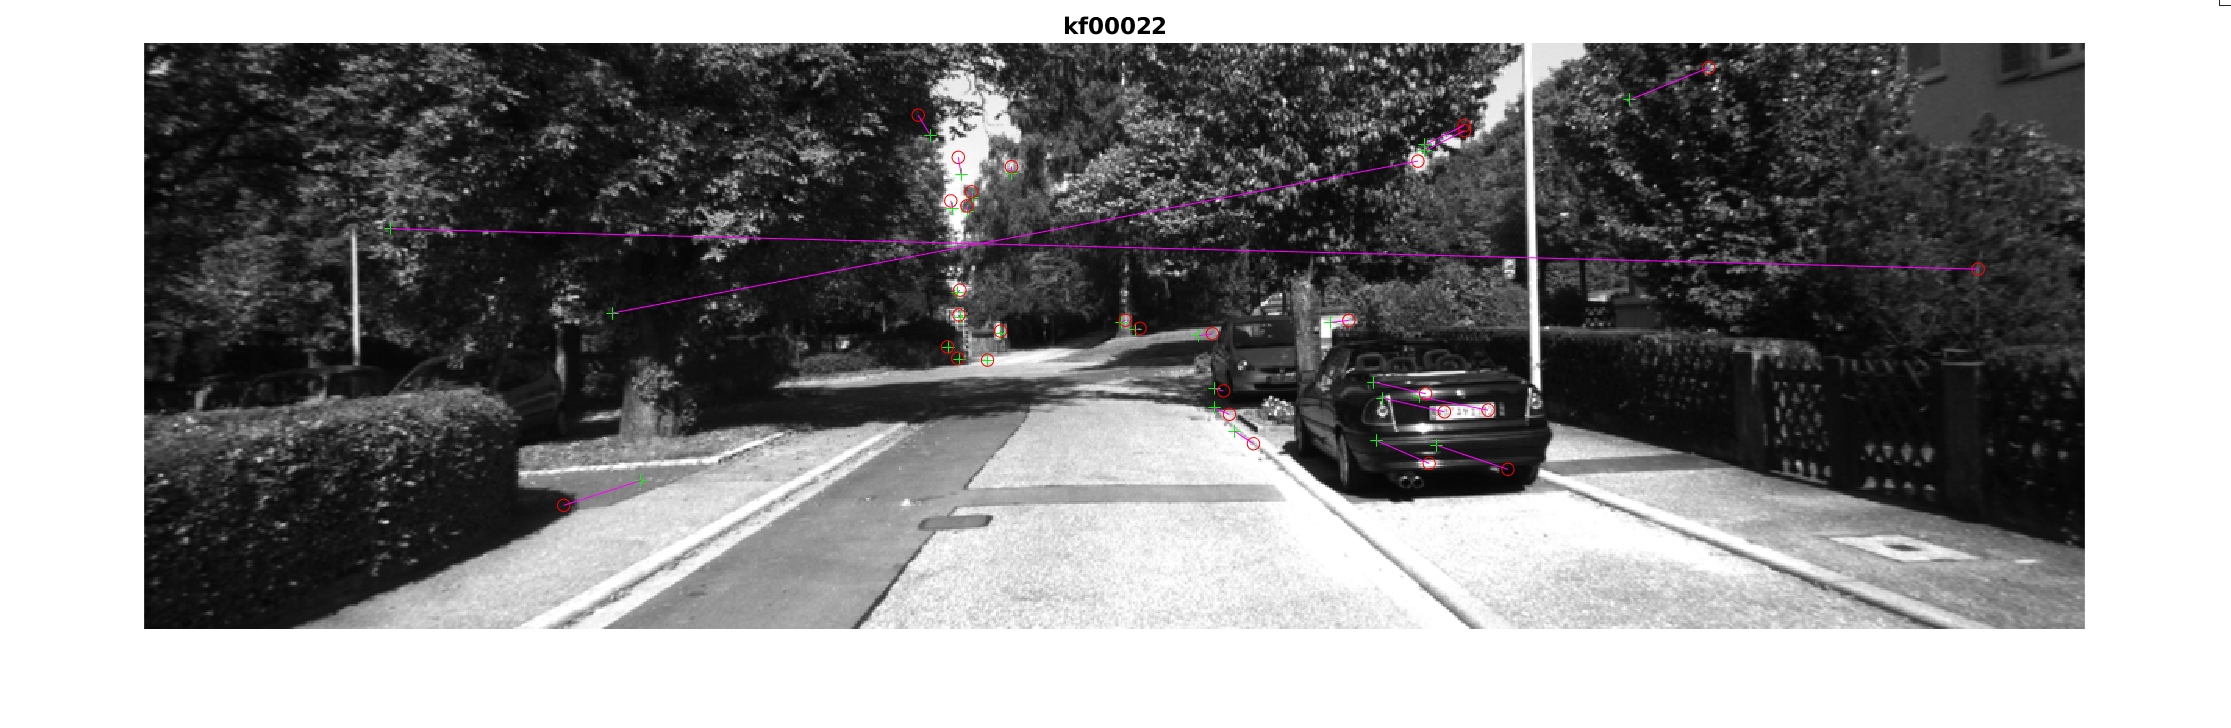
\includegraphics[width=\linewidth]{fig_mat-feat_kf00022.png}
      \end{center}
      \caption{Noisy point-feature matches between two frames.}
    \end{figure}

    \begin{figure}[H]
      \begin{center}
        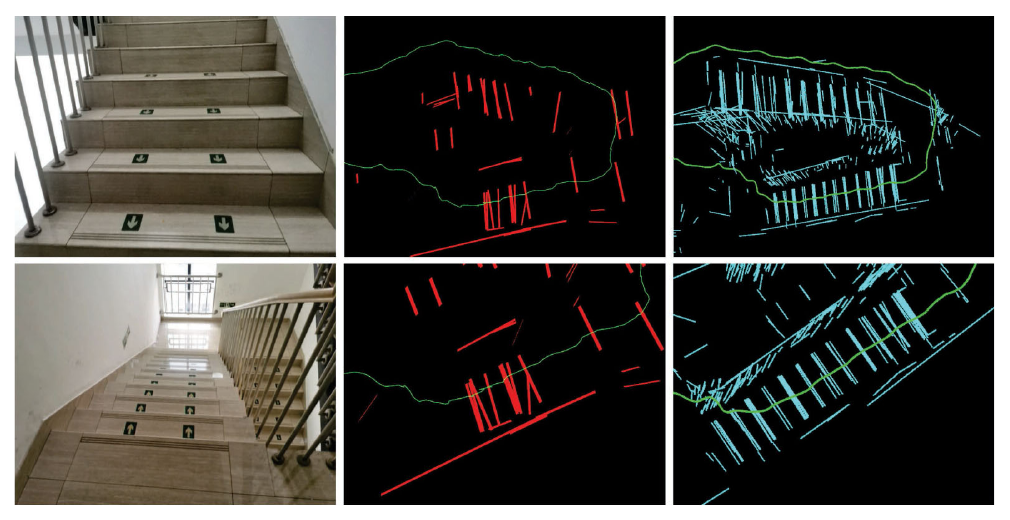
\includegraphics[width=.8\linewidth]{line_features.png}
      \end{center}
      \caption{Line-features from an image sequence.}
    \end{figure}

    \begin{figure}[H]
      \begin{center}
        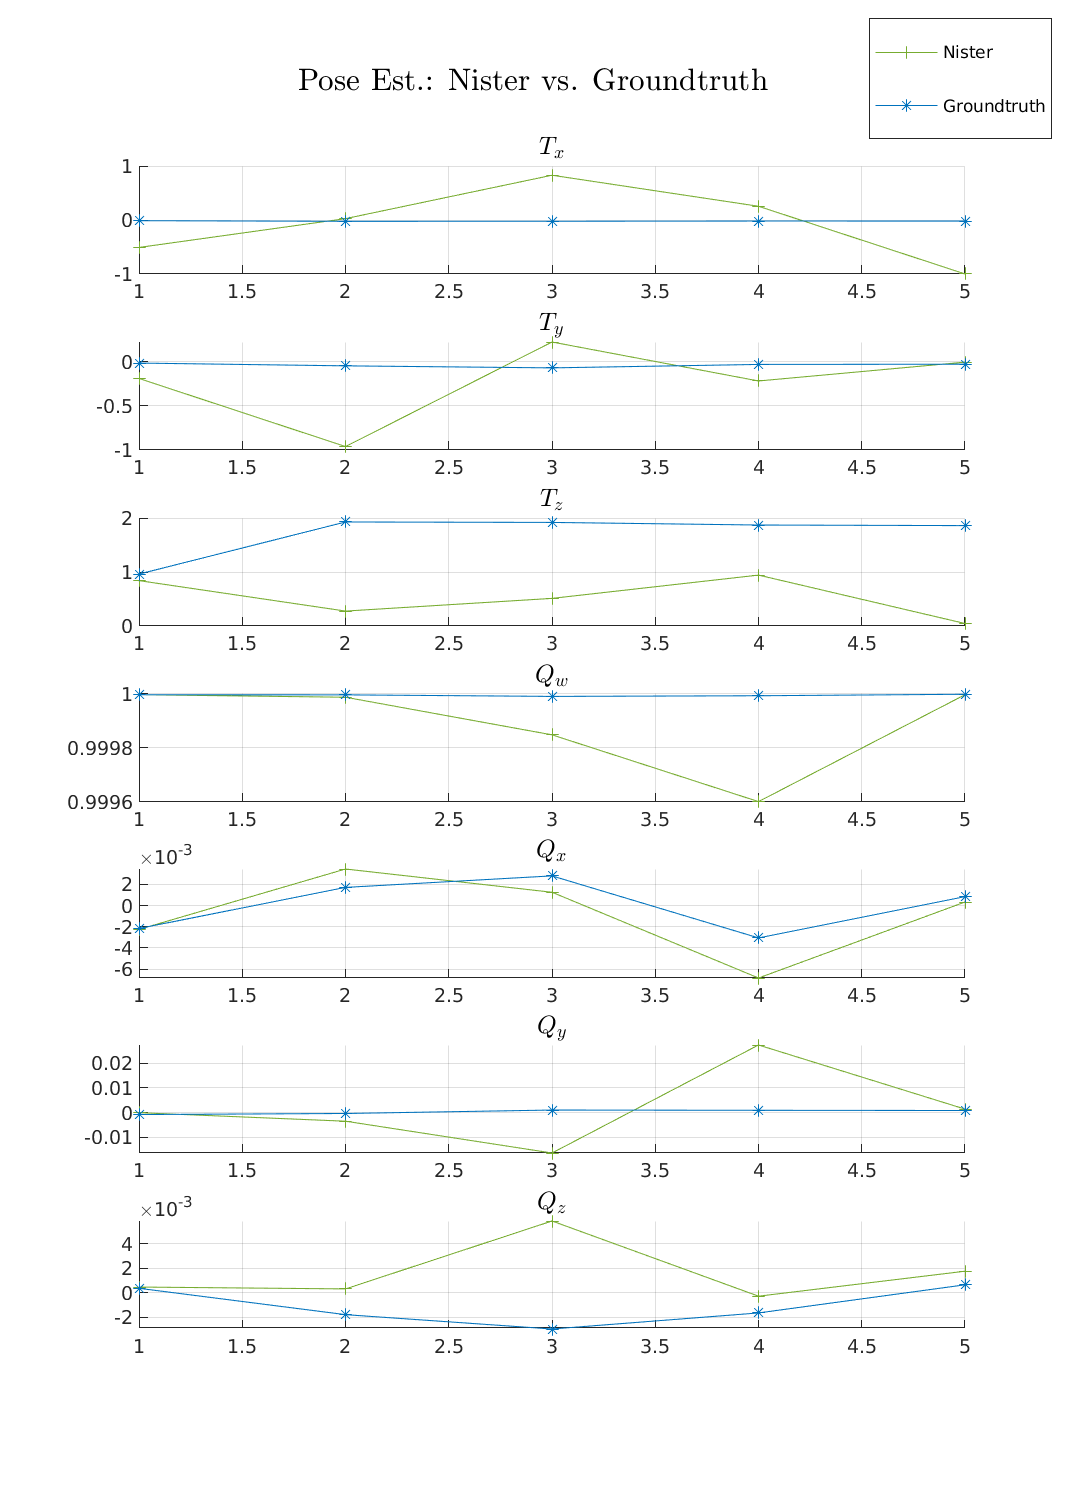
\includegraphics[width=\linewidth]{plt_pos_log_Nister.png}
      \end{center}
      \caption{Pose estimation log: Nister vs. Groundtruth.}
    \end{figure}


    \begin{figure}[H]
      \begin{center}
        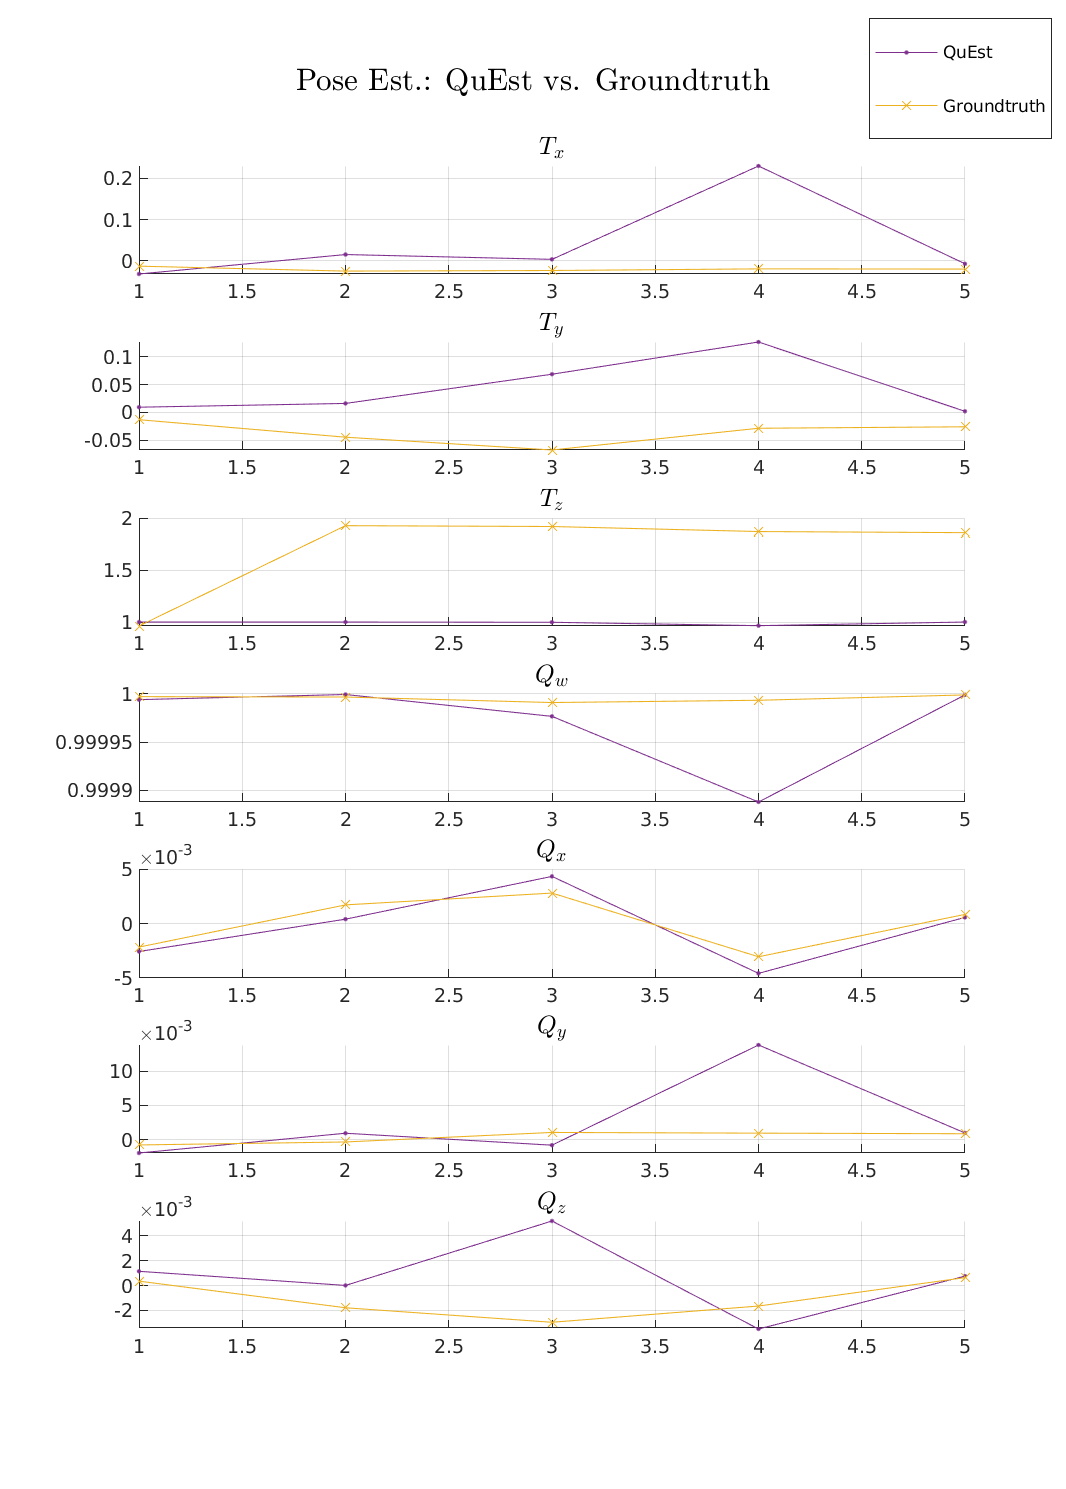
\includegraphics[width=\linewidth]{plt_pos_log_QuEst.png}
      \end{center}
      \caption{Pose estimation log: QuEst vs. Groundtruth.}
    \end{figure}

    \item XEst - Semantic segmentation (\textcolor{red}{RAL - April 30st, 2022}):
    No update on implementing \cite{ballester2021dot}.

    \item DLO Dataset: I installed Unity and soon will begin working on tutorials.
    \item Linus (REU): He is working on Unity tutorials, recreating RVL workcell,
    and importing UR5 model into Unity.
    \item Maicol (REU): He is working on ROS2 tutorials, MoveIt tutorials, and
    way-point navigation of UR5 in Unity.
    \item Myself (with REU): I will start on MuJuCo tutorials as well.

    \item DLO Control (MuJuCo): No update.

    \item Grasping Project (\textcolor{blue}{DLO-03}): I am making this a part of the DLO project.
    \item PyTorch Tutorials: Transfer learning.
    \item Manifold learning: Marcus emailed me some papers, I will read them
    and reply to him. I am not particularly interested in the project but his
    ideas are interesting and I would like to help him if I can. He is very
    knowledgeable on mathematics and I cherish that.

  \end{itemize}

\section{Intermediate Goals - Fall 2021:}
\begin{itemize}
      \item QEKF: Finish paper.
      \item UR5e: Do the tutorials.
\end{itemize}

\newpage

%Sets the bibliography style to UNSRT and import the
\newpage
\bibliography{ref}
\bibliographystyle{ieeetr}

\end{document}
